\section{Inside Heat Balance}\label{inside-heat-balance}

The heart of the heat balance method is the internal heat balance involving the inside faces of the zone surfaces.~ This heat balance is generally modeled with four coupled heat transfer components: 1) conduction through the building element, 2) convection to the air, 3) short wave radiation absorption and reflectance and 4) longwave radiant interchange.~ The incident short wave radiation is from the solar radiation entering the zone through windows and emittance from internal sources such as lights.~ The longwave radiation interchange includes the absorption and emittance of low temperature radiation sources, such as all other zone surfaces, equipment, and people.

The heat balance on the inside face can be written as follows:

\begin{equation}
{q''_{LWX}} + {q''_{SW}} + {q''_{LWS}} + {q''_{ki}} + {q''_{sol}} + {q''_{conv}} = 0
\label{eq:InsideFaceHeatBalanceEquation}
\end{equation}

where:

\({q''_{LWX}}\) = Net longwave radiant exchange flux between surfaces in a zone or group of zones (enclosure).

\({q''_{SW}}\) ~ = Net short wave radiation flux to surface from lights.

\({q''_{LWS}}\) = Longwave radiation flux from equipment in a zone or group of zones (enclosure).

\({q''_{ki}}\) ~ = Conduction flux through the wall.

\({q''_{sol}}\) ~ = Transmitted solar radiation flux absorbed at surface.

\({q''_{conv}}\) ~ = Convective heat flux to zone air.

Each of these heat balance components is introduced briefly below.

\begin{figure}[hbtp] % fig 19
\centering
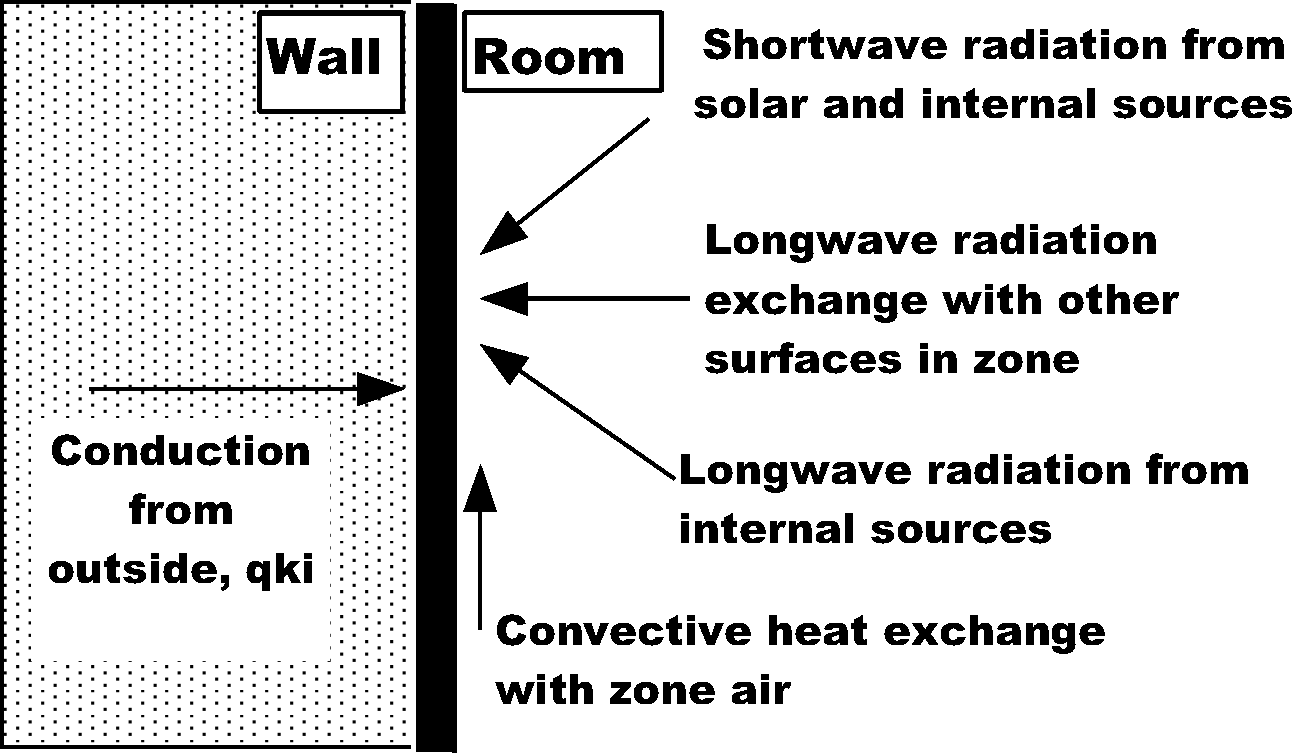
\includegraphics[width=0.9\textwidth, height=0.9\textheight, keepaspectratio=true]{media/image301.png}
\caption{Inside Heat Balance Control Volume Diagram \protect \label{fig:inside-heat-balance-control-volume-diagram}}
\end{figure}

\subsection{Internal Long-Wave Radiation Exchange}\label{internal-long-wave-radiation-exchange}

Long-wave radiation exchange is balanced within an enclosure which may be a single zone or a group of zones connected by air boundaries (see Construction:AirBoundary). Throughout this section, ``Zone'' refers to either type of enclosure.

\subsubsection{LW Radiation Exchange Among Zone Surfaces}\label{lw-radiation-exchange-among-zone-surfaces}

There are two limiting cases for internal LW radiation exchange that are easily modeled:

\begin{itemize}
\item
The zone air is completely transparent to LW radiation.
\item
The zone air completely absorbs LW radiation from the surfaces within the zone.
\end{itemize}

The limiting case of completely absorbing air has been used for load calculations and also in some energy analysis calculations.~ This model is attractive because it can be formulated simply using a combined radiation and convection heat transfer coefficient from each surface to the zone air.~ However, it oversimplifies the zone surface exchange problem, and as a result, the heat balance formulation in EnergyPlus treats air as completely transparent.~ This means that it does not participate in the LW radiation exchange among the surfaces in the zone. The model, which considers room air to be completely transparent, is reasonable physically because of the low water vapor concentrations and the short mean path lengths.~ It also permits separating the radiant and convective parts of the heat transfer at the surface, which is an important attribute of the heat balance method.

EnergyPlus uses a grey interchange model for the longwave radiation among zone surfaces. EnergyPlus offers two algorithms for modeling long wave radiation: The ``ScriptF'' method, and the ``CarrollMRT'' methods. Users can select between these two algorithms using the ``PerformancePrecisionTradeoffs'' object.

\paragraph{ScriptF}

The ``ScriptF'' algorithm was developed by Hottel (Hottel and Sarofim, Radiative Transfer, Chapter 3, McGraw Hill, 1967).~ This procedure relies on a matrix of exchange coefficients between pairs of surfaces that include all exchange paths between the surfaces.~ In other words all reflections, absorptions and re-emissions~ from other surfaces in the enclosure are included in the exchange coefficient, which is called ScriptF.~ The major assumptions are that all surface radiation properties are grey and all radiation is diffuse.~ Both assumptions are reasonable for building zone interchange.

~The ScriptF coefficients are developed by starting with the traditional direct radiation view factors.~ In the case of building rooms and zones, there are several complicating factors in finding the direct view factors---the main one being that the location of surfaces such as thermal mass representing furniture and partitions are not known.~ The other limitation is that the exact calculation of direct view factors is computationally very intensive even if the positions of all surfaces are known. Accordingly, EnergyPlus uses a procedure to approximate the direct view factors.~ The procedure has two steps:

1)~~~Determine the total area of other surfaces ``seen'' by a surface.

2)~~~Approximate the direct view factor from surface 1 to surface 2 as the ratio of the area of surface 2 to the total area ``seen'' by surface 1.

The determination of the ``seen'' area has several constraints:

\begin{itemize}
\item
  No surface sees itself.
\item
  All surfaces see thermal mass surfaces.
\item
  No surface facing within 10 degrees of another surface is seen by the other surface.
\item
  All surfaces see roofs, floors and ceilings (subject to the preceding facing direction constraint).
\end{itemize}

Because the approximate view factors may not satisfy the basic requirements of reciprocity (two surfaces should exchange equal amounts of heat in each direction), and completeness (every surface should have a direct view factor sum of 1.0), EnergyPlus does a view factor fix operation before they are used in the ScriptF determination.~ Normally both of the requirements are satisfied, but in some special situations they are not, and special rules are applied.

\begin{itemize}
\item
  If a user includes less than four surfaces in a zone, the enforcement of "completeness" is not strictly possible because it is not possible to have a completed enclosure with less than four surfaces.  In this situation, reciprocity is enforced initially and then view factors from each surface are summed.  When dealing with this few surfaces, the result of using approximate view factors is that once reciprocity is enforced that the largest surface in the zone will end up having view factors that sum up to greater than unity.  This is not physically possible.  So, to correct this and maintain completeness for one surface, the entire view factor matrix is divided by the largest summation of view factors for any surface in the zone.  By dividing the entire view factor matrix by the same value, the reciprocity established by the standard algorithm is maintained and completeness for one surface is established.  All of the other surfaces will not have view factors that sum up to unity and thus will not satisfy completeness.  However, these other surfaces will not have view factors that sum up to greater than unity thus avoiding a physically impossible situation.
\item
  When there are four or more surfaces in a zone but the area of one surface in a zone is greater than roughly (0.9) the sum of the areas of all other surfaces, reciprocity only is enforced.  Sometimes, for these very large surfaces, that enforcement of completeness without resorting to the very large surface seeing itself becomes impossible.  In these rare cases, the large surface is allowed to see itself.  Once this adjustment has been made, the calculation of the Script F values can proceed as normal via iteration until both completeness and reciprocity are satisfied.  Note that this adjustment might happen for very "flat" zones where one or two surfaces are have a much larger area than the other surfaces like a Trombe Walls, a large single-story interior areas that are modeled as a single zone, or a space where a very large internal mass element has been added.  Thermal mass surfaces also participate in internal long-wave radiation exchange and thus must have view factors calculated.
\end{itemize}

Warning messages are produced for both of these cases, and the results should be examined very carefully to ascertain that they are reasonable.~ The suggested action for the second case (the extra-large surface) is to divide the large surface into several smaller surfaces; then the enclosure will be treated as normal.

Once the ScriptF coefficients are determined, the longwave radiant exchange is calculated for each surface using:

\begin{equation}
{q_{i,j}} = {A_i}{F_{i,j}}\left( {T_i^4 - T_j^4} \right)
\end{equation}

where \textbf{\emph{F}}\(_{i,j}\) is the ScriptF between surfaces i and j.

\paragraph{CarrollMRT}

The Carroll method is an approximation of gray-body long-wave radiation exchange within an enclosure that simplifies the surface-to-surface radiation exchange by using a single, mean radiant temperature node, $Tr$, that acts as a clearinghouse for the radiation heat exchange between surfaces. Instead of solving a dense-matrix, linear algebra problem, the mean radiant temperature can be calculated using a single equation, and subsequently used to determine the net long-wave radiation to/from each surface. Unlike the $O(n^2)$ complexity of the current dense-matrix solution, this approach has linear complexity.

The mean radiant temperature is calculated using three steps:

\begin{enumerate}
\item Calculation of the mean radiant temperature ``view factor'', $Fi$. These view factors represent each surface's ``view'' to the mean radiant temperature node as though all surfaces were part of a spherical enclosure (i.e., they all have equal view of the node regardless of their orientation to each other). $Fi$ is calculated as:

\begin{equation}
    F_i=\frac{1}{1-\frac{A_i F_i}{\sum_1^n{A_j F_j} }}
\end{equation}

Because of the circular reference in this equation, the collection of all ``view factors'' must be solved iteratively, but only once per simulation as surface areas do not change throughout. This converges for realistic enclosures but won't necessarily converge for ``enclosures'' having only two or three surfaces, particularly if there are large area disparities.

\item Calculating the gray-body radiation resistance, $F'i$. This calculation must be computed every time surface emissivity changes. $F'i$ is calculated as:

\begin{equation}
    F'_i=\frac{\sigma\varepsilon_i}{\frac{\varepsilon_i}{F_i} +1-\varepsilon_i}
\end{equation}

\item Finally, the mean radiant temperature, $Tr$, is:

\begin{equation}
    T_r=\frac{\sum_1^nA_i F'_i T_i}{\sum_1^nA_i F'_i}
\end{equation}

\end{enumerate}

Once the mean radiant temperature is known, the net radiation heat transfer for each surface can be calculated as:

\begin{equation}
    q=F'_i A_i (T_r^4-T_i^4)
\end{equation}

Carroll, J. A., 1980, ``An `MRT Method' of Computing Radiant Energy Exchange in Rooms,'' Proceedings of the Second Systems Simulation and Economic Analysis Conference, San Diego, CA.

Carroll, J. A., 1980a, ``An MRT method of computing radiant energy exchange in rooms,'' Proceedings of the 2nd Systems Simulation and Economic Analysis Conference, San Diego, CA.

Carroll, J. A., 1981, ``A Comparison of Radiant Interchange Algorithms,'' Proceedings of the 3rd Annual Systems Simulation and Economics Analysis/Solar Heating and Cooling Operational Results Conference, Reno. Solar Engineering, Proceedings of the ASME Solar division.


\subsubsection{Thermal Mass and Furniture}\label{thermal-mass-and-furniture}

Furniture in a zone has the effect of increasing the amount of surface area that can participate in the radiation and convection heat exchanges.~ It also adds participating thermal mass to the zone.~ These two changes both affect the response to temperature changes in the zone and also affect the heat extraction characteristics.

The proper modeling of furniture is an area that needs further research, but the heat balance formulation allows the effect to be modeled in a realistic manner by including the furniture surface area and thermal mass in the heat exchange process.

\subsubsection{LW Radiation From Internal Sources}\label{lw-radiation-from-internal-sources}

The traditional model for this source is to define a radiative/convective split for the heat introduced into a zone from equipment.~ The radiative part is then distributed over the surfaces within the zone in some prescribed manner.~ This, of course, is not a completely realistic model, and it departs from the heat balance principles. However, it is virtually impossible to treat this source in any more detail since the alternative would require knowledge of the placement and surface temperatures of all equipment.

\subsection{Internal Short-Wave Radiation}\label{internal-short-wave-radiation}

\subsubsection{SW Radiation from Lights}\label{sw-radiation-from-lights}

The short wavelength radiation from lights is distributed over the surfaces in the zone in some prescribed manner.

\subsubsection{Transmitted Solar}\label{transmitted-solar}

Transmitted solar radiation is also distributed over the surfaces in the zone in a prescribed manner.~ It would be possible to calculate the actual position of beam solar radiation, but that would involve partial surface irradiation, which is inconsistent with the rest of the zone model that assumes uniform conditions over an entire surface.~ The current procedures incorporate a set of prescribed distributions.~ Since the heat balance approach can deal with any distribution function, it is possible to change the distribution function if it seems appropriate.

\subsubsection{Convection to Zone Air}\label{convection-to-zone-air}

The convection flux is calculated using the heat transfer coefficients as follows:

\begin{equation}
{q''_{conv}} = {h_c}({T_s} - {T_a})
\end{equation}

The inside convection coefficients (\emph{h\(_{c}\)}) can be calculated using one of many different models.~ Currently the implementation uses coefficients based on correlations for natural, mixed, and forced convection.

\subsection{Interior Conduction}\label{interior-conduction}

This contribution to the inside surface heat balance is the wall conduction term, \({q''_{ki}}\) ~shown in Equation~\ref{eq:InsideFaceHeatBalanceEquation}. This represents the heat transfer to the inside face of the building element. Again, a CTF formulation is used to determine this heat flux.

\subsection{Interior Convection}\label{interior-convection}

There are many different modeling options available in EnergyPlus for inside convection coefficients, \emph{h\(_{c}\)}.~ There are four different settings to direct how EnergyPlus managers select \emph{h\(_{c}\)} models during a simulation.~ There are numerous individual model equations for \emph{h\(_{c}\)} in EnergyPlus to cover different situations that arise from surface orientations, room airflow conditions, and heat flow direction.~ Additionally, in many cases multiple researchers have developed competing models for the same situations that differ and there is no way to declare one is better than another.~ An overall default for the simulation is selected in the ``SurfaceConvectionAlgorithm:Inside'' object and can be overridden by selecting a different option in a zone description.~ These models are explained in the following sections. In addition to the correlation choices described below, it is also possible to override the convection coefficients on the inside of any surface by using the ``SurfaceProperty:ConvectionCoefficients'' object in the input file to set the convection coefficient value on the inside of any surface. The values can be specified directly or with schedules. Specific details are given in the Input Output Reference document.

For exterior simple-glazing windows modeled with the WindowMaterial:SimpleGlazingSystem
object, \emph{h\(_{c}\)} is scaled with an adjustment ratio. This enables the modeling
of simple windows with highly conductive frames (large input U values). The calculation
of the adjustment ratio is detailed in Section~\ref{application-issues}.

\subsubsection{Adaptive Convection Algorithm}\label{adaptive-convection-algorithm}

Beausoleil-Morrison (2000, 2002) developed a methodology for dynamically managing the selection of \emph{h\(_{c}\)} equations called \emph{adaptive convection algorithm}.~ The algorithm is used to select among the available \emph{h\(_{c}\)} equations for the one that is most appropriate for a given surface at a given time.~ As Beausoleil-Morrison notes, the adaptive convection algorithm is intended to be expanded and altered to reflect different classification schemes and/or new \emph{h\(_{c}\)} equations.~ The implementation in EnergyPlus has been modified from the original in the following ways:

\begin{itemize}
\item
  An input mechanism is provided (see the \\
SurfaceConvectionAlgorithm:Inside:AdapativeModelSelections object) so that the user can customize the specific selections of \emph{h\(_{c}\)} equations that are applied for different flow regimes and surface orientations.~ The changes apply in a general way to the entire model (but can be overridden by setting surface properties).
\item
  To avoid requiring additional user input on the position of ZoneHVAC-type equipment within a zone, there is no distinction between zones that have convective zone heater equipment located underneath the windows and those that have convective heaters located away from the windows.~ This applies to the air flow regime associated with convective zone heaters.~ Using Beausoleil-Morrison's terminology, regimes B1 and B2 are combined into just one B regime.
\item
  To avoid requiring additional user input on the position of ZoneHVAC-type equipment within a zone, there is no distinction between surfaces that are directly blown on the fan and those that are away from the fan for the air flow regime associated with mechanical circulation from a zone fan (ZoneHVAC type equipment).
\item
  The correlation for horizontal free jet developed by Fisher (1995) is not used.~ Ceiling diffuser models are used for all mechanical circulation from central air system.~ This decision was made for two reasons: (1) to avoid requiring additional user input on the position of, and momentum generated by, air terminal units, and (2) because Fisher (1995) found that the Coanda effect is so significant that in practice a free horizontal jet is difficult to maintain and mechanical-driven room airflows generally attach to surfaces and tend to match the flow regime of a ceiling diffuser much more often than a free jet.
\item
  EnergyPlus supports arbitrary geometry so surfaces can be tilted with respect to vertical or horizontal.~ Beausoleil-Morrison's adaptive convection algorithm was originally structured to use \emph{h\(_{c}\)} equations that have no functional dependence on surface tilt angle.~ However, tilted surfaces do perform differently than vertical or horizontal surface when buoyancy forces are significant.~ Therefore, the EnergyPlus implementation expands the structure of the algorithm to include additional categories for tilted surfaces.~ The \emph{h\(_{c}\)} equations developed by Walton (1983) are selected as the defaults for tilted surfaces because they have a functional dependence on tilt angle.
\item
  Fohanno and Polidari (2006) produced a new \emph{h\(_{c}\)} equation for vertical walls inside buildings with a simple buoyancy flow regime.~ They used a theoretical approach based on integral formalism and uniform heat flux (rather than uniform temperature) that covers both laminar and turbulent flow situations. ~In EnergyPlus, this model is selected as the default in place of the model by Alamdari and Hammond (1983) for vertical walls.
\item
  Karadag (2009) produced a new \emph{h\(_{c}\)} equation for ceiling surfaces that are actively chilled.~ He used computation fluid dynamics and various sized rooms and temperature conditions.~ In EnergyPlus, this model is selected as the default for surfaces that have active, in-ceiling cooling (in place of the model by Alamdari and Hammond (1983) for unstable ceilings).
\item
  International Standard Organization (ISO) completed Standard 15099-2003 which includes \emph{h\(_{c}\)} equations for the inside face of windows.~ EnergyPlus strives to adhere to formal modeling Standards where possible.~ Therefore the implementation includes a larger structure for the adaptive algorithm that includes additional categories for windows in all flow regimes and ISO 15099-2003 models are used as the default for windows in natural convection flow regimes.~ The ISO 15099 model applies to various tilt angles.
\item
  Goldstein and Novosalec (2010) produced new \emph{h\(_{c}\)} equations for forced air situations with ceiling slot diffusers along perimeters with significant glazing fractions.~ They used experiments with full-sized test room.~ These new equations are selected as the default for windows, ceilings and floors when there is an active central air system.
\item
  Interior mass surfaces are assigned the \emph{h\(_{c}\)} equation that would apply (stable or unstable) to a horizontal, upward facing surface for each flow regime.
\item
  The algorithm switches between forced, mixed, and natural flow regimes by calculating the Richardson number, Ri = Gr/Re\^{}2, for the zone.~ Large values of Ri indicate buoyancy dominates, while small values indicate forced flows dominate. To distinguish between opposing Zone unit type equipment (with fans) are assumed to force air up walls, and central air type equipment (with diffusers) are assumed to force air down walls.
\end{itemize}

The adaptive convection algorithm implemented in EnergyPlus for the inside face has a total of 45 different categories for surfaces and 29 different options for \emph{h\(_{c}\)} equation selections.~ The following table summarizes the categories and the default assignments for \emph{h\(_{c}\)} equations.~ The individual \emph{h\(_{c}\)} equations are documented below.

{\scriptsize
\begin{longtable}[c]{p{0.25in}p{1.25in}p{0.25in}p{1.5in}p{2.5in}}

\caption{Inside Convection Categories and Assignments \label{table:table-13.-inside-convection-categories}} \tabularnewline
\toprule 
\# & Zone Air Flow Regime & IB-M's \# & Surface orientation and heat flow direction & Keywords for Applicable Model Equation Sources \tabularnewline
\midrule
\endfirsthead

\caption[]{Inside Convection Categories and Assignments} \tabularnewline
\toprule 
\# & Zone Air Flow Regime & IB-M's \# & Surface orientation and heat flow direction & Keywords for Applicable Model Equation Sources \tabularnewline
\midrule
\endhead

1  & & & Vertical Walls & FohannoPolidoriVerticalWall* \tabularnewline
   & & & & AlamdariHammondVerticalWall \tabularnewline
   & & & & ASHRAEVerticalWall \tabularnewline
2  & & & Stable Horizontal & AlamdariHammondStableHorizontal* \tabularnewline
   & & & & WaltonStableHorizontalOrTilt \tabularnewline
3  & Simple Buoyancy & A3 & Unstable Horizontal & AlamdariHammondUnstableHorizontal* \tabularnewline
   & & & & WaltonUnstableHorizontalOrTilt \tabularnewline
4  & & & Stable Tilted & WaltonStableHorizontalOrTilt* \tabularnewline
5  & & & Unstable Tilted & WaltonUnstableHorizontalOrTilt* \tabularnewline
6  & & & Windows & ISO15099Windows* \tabularnewline
\midrule
7  & & & Vertical Walls & KhalifaEq3WallAwayFromHeat* \tabularnewline
   & & & & FohannoPolidoriVerticalWall \tabularnewline
   & & & & AlamdariHammondVerticalWall \tabularnewline
   & & & & ASHRAEVerticalWall \tabularnewline
8  & & & Stable Horizontal & AlamdariHammondStableHorizontal* \tabularnewline
   & & & & WaltonStableHorizontalOrTilt \tabularnewline
9  & In-floor Heating or In-ceiling Cooling & A1 & Unstable Horizontal & KhalifaEq4CeilingAwayFromHeat* \tabularnewline
   & & & & AlamdariHammondUnstableHorizontal \tabularnewline
   & & & & WaltonUnstableHorizontalOrTilt \tabularnewline
10 & & & Heated Floor & AwbiHattonHeatedFloor* \tabularnewline
 & & & & WaltonUnstableHorizontalOrTilt \tabularnewline
 & & & & AlamdariHammondUnstableHorizontal \tabularnewline
11 & & & Chilled Ceiling & KaradagChilledCeiling* \tabularnewline
 & & & & WaltonUnstableHorizontalOrTilt \tabularnewline
12 & & & Stable Tilted & WaltonStableHorizontalOrTilt* \tabularnewline
13 & & & Unstable Tilted & WaltonUnstableHorizontalOrTilt* \tabularnewline
14 & & & Windows & ISO15099Windows* \tabularnewline
\midrule
15 & & & Vertical Walls (non-heated) & KhalifaEq6NonHeatedWalls* \tabularnewline
 & & & & FohannoPolidoriVerticalWall \tabularnewline
 & & & & ASHRAEVerticalWall \tabularnewline
16 & & & Heated Wall & AwbiHattonHeatedWall* \tabularnewline
17 & Wall Panel Heating & A2 & Stable Horizontal & AlamdariHammondStableHorizontal* \tabularnewline
 & & & & WaltonStableHorizontalOrTilt \tabularnewline
18 & & & Unstable Horizontal & KhalifaEq7Ceiling* \tabularnewline
 & & & & AlamdariHammondUnstableHorizontal \tabularnewline
 & & & & WaltonUnstableHorizontalOrTilt \tabularnewline
19 & & & Stable Tilted & WaltonStableHorizontalOrTilt* \tabularnewline
20 & & & Unstable Tilted & WaltonUnstableHorizontalOrTilt* \tabularnewline
21 & & & Windows & ISO15099Windows* \tabularnewline
\midrule
22 & & & Vertical Walls not near heater & FohannoPolidoriVerticalWall* \tabularnewline
 & & & & KhalifaEq6NonHeatedWalls \tabularnewline
 & & & & KhalifaEq3WallAwayFromHeat \tabularnewline
 & & & & AlamdariHammondVerticalWall \tabularnewline
 & & & & ASHRAEVerticalWall \tabularnewline
23 & & & Vertical Walls near heater & KhalifaEq5WallNearHeat* \tabularnewline
24 & Convective Zone Heater & B & Stable Horizontal & AlamdariHammondStableHorizontal* \tabularnewline
 & & & & WaltonStableHorizontalOrTilt \tabularnewline
25 & & & Unstable Horizontal & KhalifaEq7Ceiling* \tabularnewline
 & & & & KhalifaEq4CeilingAwayFromHeat \tabularnewline
 & & & & WaltonUnstableHorizontalOrTilt \tabularnewline
26 & & & Stable Tilted & WaltonStableHorizontalOrTilt* \tabularnewline
27 & & & Unstable Tilted & WaltonUnstableHorizontalOrTilt* \tabularnewline
28 & & & Windows & ISO15099Windows* \tabularnewline
\midrule
29 & & & Walls & GoldsteinNovoselacCeilingDiffuserWalls* \tabularnewline
 & & & & FisherPedersenCeilingDiffuserWalls \tabularnewline
30 & & & Ceiling & FisherPedersenCeilingDiffuserCeiling* \tabularnewline
31 & Mechanical Central Air Diffuser & C & Floor & GoldsteinNovoselacCeilingDiffuserFloor* \tabularnewline
 & & & & FisherPedersenCeilingDiffuserFloor \tabularnewline
32 & & & Windows & GoldsteinNovoselacCeilingDiffuserWindow* \tabularnewline
 & & & & ISO15099Windows \tabularnewline
\midrule
33 & & & Walls & KhalifaEq3WallAwayFromHeat * \tabularnewline
34 & & & Stable Horizontal & AlamdariHammondStableHorizontal* \tabularnewline
 & & & & WaltonStableHorizontalOrTilt \tabularnewline
35 & Mechanical Zone Fan Circulation & D & Unstable Horizontal & KhalifaEq4CeilingAwayFromHeat* \tabularnewline
 & & & & WaltonUnstableHorizontalOrTilt \tabularnewline
36 & & & Stable Tilted & WaltonStableHorizontalOrTilt* \tabularnewline
37 & & & Unstable Tilted & WaltonUnstableHorizontalOrTilt* \tabularnewline
38 & & & Windows & GoldsteinNovoselacCeilingDiffuserWindow* \tabularnewline
 & & & & ISO15099Windows \tabularnewline
\midrule
39 & & & Assisting Flow Walls & BeausoleilMorrisonMixedAssistedWall* \tabularnewline
40 & & & Opposing Flow Walls & BeausoleilMorrisonMixedOpposingWall* \tabularnewline
41 & & & Stable Floor & BeausoleilMorrisonMixedStableFloor* \tabularnewline
42 & Mixed & E & Unstable Floor & BeausoleilMorrisonMixedUnstableFloor* \tabularnewline
43 & & & Stable Ceiling & BeausoleilMorrisonMixedStableCeiling* \tabularnewline
44 & & & Unstable Ceiling & BeausoleilMorrisonMixedUnstableCeiling* \tabularnewline
45 & & & Windows & GoldsteinNovoselacCeilingDiffuserWindow* \tabularnewline
 & & & & ISO15099Windows \tabularnewline
\bottomrule
\end{longtable}}

*Indicates the default selection for \emph{h\(_{c}\)} model equation.

\subsubsection{Inside Face Surface Classification}\label{inside-face-surface-classification}

The adaptive convection algorithm is based on classifying surfaces by flow regime and orientation so that the correct \emph{h\(_{c}\)} equation can be chosen at a particular point in time during the simulation.~ The classification depends on user input with some aspects processed only once at the beginning and others during each timestep.~ There are also various parameters or inputs to the \emph{h\(_{c}\)} equations that need static or dynamic processing.

For each surface, it and the zone it is attached to are processed for the following static characteristics.

\begin{itemize}
\item
  Characteristic height for convection is taken as the zone height.
\item
  Surfaces listed as receiving heat from Zone HVAC equipment with radiative models are considered ``near'' the heater.
\item
  Zones are examined for low temperature radiant systems.~ The surfaces that contain the active elements are examined and the zone characterized to know if it has in-floor heating, in-ceiling cooling, or in-wall heating.
\item
  A hydraulic diameter is calculated for horizontal surfaces for the entire zone.
\end{itemize}

and calculating various parameters needed by \emph{h\(_{c}\)} equations.~ Selecting flow regime is done in the following manner.~ For each surface, we examine the zone on the inside face for the following:

\begin{itemize}
\item
  HVAC system type
\item
  HVAC operating status
\item
  HVAC system ACH
\end{itemize}

During initial zone and system sizing calculations, HVAC system characteristics are not known yet, so the flow regime is selected assuming an uncontrolled zone. During simulations, including HVAC sizing simulations, the HVAC system characteristics are used.

The surfaces are evaluated to determine:

\begin{itemize}
\item
  Surface classification: Floor, wall, roof, window, types
\item
  Tilt angle
\item
  Convective stability (sign of ΔT)
\end{itemize}

The individual \emph{h\(_{c}\)} model equations and their respective references are listed in next by the keyword used to identify them.

\subsubsection{ASHRAE Vertical Wall}\label{ashrae-vertical-wall}

Walton adopted the following equation for natural convection from ASHRAE .

\begin{equation}
h = 1.31{\left| {\Delta T} \right|^{\frac{1}{3}}}
\end{equation}

This is usually bound at a minimum of .1 in EnergyPlus. This is a component of the TARP overall algorithm described below.

\subsubsection{Walton Unstable Horizontal Or Tilt}\label{walton-unstable-horizontal-or-tilt}

Walton (1983) developed the following equation by fitting curves from various sources.

\begin{equation}
h = \frac{{9.482{{\left| {\Delta T} \right|}^{\frac{1}{3}}}}}{{7.238 - \left| {\cos \Sigma } \right|}}
\end{equation}

Unstable refers to the direction of heat flow and the associated buoyancy relative to the surfaces. Unstable is when the natural tendency is to enhance flow in the sense that rising warmer air, or falling cooler air, is free to move away from the surface. This is usually bound at a minimum of .1 in EnergyPlus. This is a component of the TARP overall algorithm described below.

\subsubsection{Walton Stable Horizontal Or Tilt}\label{walton-stable-horizontal-or-tilt}

Walton (1983) developed the following equation by fitting curves from various sources.

\begin{equation}
h = \frac{{1.810{{\left| {\Delta T} \right|}^{\frac{1}{3}}}}}{{1.382 + \left| {\cos \Sigma } \right|}}
\end{equation}

Stable refers to the direction of heat flow and the associated buoyancy relative to the surfaces. Stable is when the natural tendency is to retard flow in the sense that rising warmer air, or falling cooler air, is driven against the surface. This is usually bound at a minimum of .1 in EnergyPlus. This is a component of the TARP overall algorithm described below.

\subsubsection{Fisher Pedersen Ceiling Diffuser Walls}\label{fisher-pedersen-ceiling-diffuser-walls}

Fisher and Pedersen (1997) developed the following equation from laboratory chamber measurements.

\begin{equation}
h = 1.208 + 1.012 * AC{H^{0.604}}
\end{equation}

This is a component of the CeilingDiffuser overall algorithm described below.

\subsubsection{Fisher Pedersen Ceiling Diffuser Ceiling}\label{fisher-pedersen-ceiling-diffuser-ceiling}

Fisher and Pedersen (1997) developed the following equation from laboratory chamber measurements.

\begin{equation}
h = 2.234 + 4.099 * AC{H^{0.503}}
\end{equation}

This is a component of the CeilingDiffuser overall algorithm described below.

\subsubsection{Fisher Pedersen Ceiling Diffuser Floor}\label{fisher-pedersen-ceiling-diffuser-floor}

Fisher and Pedersen (1997) developed the following equation from laboratory chamber measurements.

\begin{equation}
h = 3.873 + 0.082 * AC{H^{0.98}}
\end{equation}

This is a component of the CeilingDiffuser overall algorithm described below.

\subsubsection{Alamdari Hammond Stable Horizontal}\label{alamdari-hammond-stable-horizontal}

Alamdari and Hammond (1983) developed the following correlation for horizontal surfaces in stable thermal situation.

\begin{equation}
h = 0.6{\left( {\frac{{\left| {\Delta T} \right|}}{{D_h^2}}} \right)^{{\raise0.7ex\hbox{1} \!\mathord{\left/ {\vphantom {1 5}}\right.}\!\lower0.7ex\hbox{5}}}}
\end{equation}

where,

\({D_h} = \frac{{4A}}{P}\) , hydraulic diameter of horizontal surface, \emph{A} is area (m\(^{2}\)) and \emph{P} is the perimeter (m) of the entire zone.

\subsubsection{Alamdari Hammond Unstable Horizontal}\label{alamdari-hammond-unstable-horizontal}

Alamdari and Hammond (1983) developed the following correlation for horizontal surfaces in a buoyant thermal situation.

\begin{equation}
h = {\left\{ {{{\left[ {1.4{{\left( {\frac{{\left| {\Delta T} \right|}}{{{D_h}}}} \right)}^{^{{\raise0.7ex\hbox{1} \!\mathord{\left/ {\vphantom {1 4}}\right.}\!\lower0.7ex\hbox{4}}}}}} \right]}^6} + {{\left[ {1.63{{\left| {\Delta T} \right|}^{{\raise0.7ex\hbox{1} \!\mathord{\left/ {\vphantom {1 3}}\right.}\!\lower0.7ex\hbox{3}}}}} \right]}^6}} \right\}^{{\raise0.7ex\hbox{1} \!\mathord{\left/ {\vphantom {1 6}}\right.}\!\lower0.7ex\hbox{6}}}}
\end{equation}

\subsubsection{Alamdari Hammond Vertical Wall}\label{alamdari-hammond-vertical-wall}

Alamdari and Hammond (1983) developed the following correlation for vertical surfaces.

\begin{equation}
h = {\left\{ {{{\left[ {1.5{{\left( {\frac{{\left| {\Delta T} \right|}}{H}} \right)}^{^{{\raise0.7ex\hbox{1} \!\mathord{\left/ {\vphantom {1 4}}\right.}\!\lower0.7ex\hbox{4}}}}}} \right]}^6} + {{\left[ {1.23{{\left| {\Delta T} \right|}^{{\raise0.7ex\hbox{1} \!\mathord{\left/ {\vphantom {1 3}}\right.}\!\lower0.7ex\hbox{3}}}}} \right]}^6}} \right\}^{{\raise0.7ex\hbox{1} \!\mathord{\left/ {\vphantom {1 6}}\right.}\!\lower0.7ex\hbox{6}}}}
\end{equation}

where,

~~~~~ \emph{H} is the characteristic height for the surface.~ In EnergyPlus this is the zone's ceiling height (which could be larger than the height of an individual surface when wall are subdivided into more than one surface).

\subsubsection{Khalifa Eq3 Wall Away From Heat}\label{khalifa-eq3-wall-away-from-heat}

Khalifa (1989) conducted experiments with test chambers and developed correlations for certain types of surfaces.~ One of them, identified as ``Equation 3'' in original reference, is for convectively heated zones and applies to the inside surfaces of walls away from the heat source:

\begin{equation}
h = 2.07{\left| {\Delta T} \right|^{0.23}}
\end{equation}

\subsubsection{Khalifa Eq4 Ceiling Away From Heat}\label{khalifa-eq4-ceiling-away-from-heat}

Khalifa (1989) conducted experiments with test chambers and developed correlations for certain types of surfaces.~ One of them, identified as ``Equation 4'' in original reference, is for convectively heated zones and applies to the inside surfaces of ceilings away from the heat source:

\begin{equation}
h = 2.72{\left| {\Delta T} \right|^{0.13}}
\end{equation}

\subsubsection{Khalifa Eq5 Wall Near Heat}\label{khalifa-eq5-wall-near-heat}

Khalifa (1989) conducted experiments with test chambers and developed correlations for certain types of surfaces.~ One of them, identified as ``Equation 5'' in original reference, is for convectively heated zones and applies to the inside surfaces of walls near the heat source:

\begin{equation}
h = 1.98{\left| {\Delta T} \right|^{0.32}}
\end{equation}

\subsubsection{Khalifa Eq6 Non Heated Walls}\label{khalifa-eq6-non-heated-walls}

Khalifa (1989) conducted experiments with test chambers and developed correlations for certain types of surfaces.~ One of them, identified as ``Equation 6'' in original reference, is for heated zones and applies to the inside surfaces of walls that are not heated:

\begin{equation}
h = 2.30{\left| {\Delta T} \right|^{0.24}}
\end{equation}

\subsubsection{Khalifa Eq7 Ceiling}\label{khalifa-eq7-ceiling}

Khalifa (1989) conducted experiments with test chambers and developed correlations for certain types of surfaces.~ One of them, identified as ``Equation 7'' in original reference, is for heated zones and applies to the inside surfaces of ceilings:

\begin{equation}
h = 3.10{\left| {\Delta T} \right|^{0.17}}
\end{equation}

\subsubsection{Awbi Hatton Heated Floor}\label{awbi-hatton-heated-floor}

Awbi and Hatton (1999) conducted laboratory measurements using environmental chambers and developed the following correlation for floor surfaces that are being actively heated.

\begin{equation}
h = \frac{{2.175{{\left| {\Delta T} \right|}^{0.308}}}}{{D_h^{0.076}}}
\end{equation}

where,

\({D_h} = \frac{{4A}}{P}\), hydraulic diameter of horizontal surface, \emph{A} is area (m\(^{2}\)) and \emph{P} is the perimeter (m) of the entire zone (all of the adjacent floor surfaces if more than one in the zone).

\subsubsection{Awbi Hatton Heated Wall}\label{awbi-hatton-heated-wall}

Awbi and Hatton (1999) developed the following correlation for wall surfaces that are being actively heated.

\begin{equation}
h = \frac{{1.823{{\left| {\Delta T} \right|}^{0.293}}}}{{D_h^{0.076}}}
\end{equation}

where,

\({D_h} = \frac{{4A}}{P}\), hydraulic diameter of wall surface, \emph{A} is area (m\(^{2}\)) and \emph{P} is the perimeter (m) of the entire wall (all of the adjacent wall surfaces if more than one along the wall).

\subsubsection{Beausoleil Morrison Mixed Assisted Wall}\label{beausoleil-morrison-mixed-assisted-wall}

Beausoleil-Morrison (2000) used blending techniques to combine correlations originally developed by Alamdari and Hammond (1983) and Fisher and Pedersen (1997) to create the following correlation is for walls where the flow driving forces from mechanical forces are augmented by the driving forces from buoyancy.

\begin{equation}
\medmuskip=0mu
\thinmuskip=0mu
\thickmuskip=0mu
\nulldelimiterspace=0pt
\scriptspace=0pt
h = \left( 
\left\{
\left[1.5\left(\frac{\left|\Delta T\right|}{H}\right)^{1/4}\right]^6 +
\left[1.23\left|\Delta T\right|^2\right]^{1/6}
\right\}^{1/2} + 
\left\{
\left[\frac{T_{surf}-T_{SAT}}{\left|\Delta T\right|}\right]
\left[-0.199+0.190\cdot ACH^{0.8}\right]
\right\}^3
\right)^{1/3}
\end{equation}

where,

~~~~~ \emph{T\(_{SAT}\)} is the supply air temperature at the diffuser.

Here the reference temperature is the zone air temperature rather than the diffuser supply air temperature.

\subsubsection{Beausoleil Morrison Mixed Opposing Wall}\label{beausoleil-morrison-mixed-opposing-wall}

Beausoleil-Morrison (2000) used blending techniques to combine correlations originally developed by Alamdari and Hammond (1983) and Fisher and Pedersen (1997) to create the following correlation is for walls where the flow driving forces from mechanical forces are opposed by the driving forces from buoyancy.

\begin{equation}
\medmuskip=0mu
\thinmuskip=0mu
\thickmuskip=0mu
\nulldelimiterspace=0pt
\scriptspace=0pt
h = \max \left\{
\begin{array}{l}
\left(\left\{\left[1.5\left(\frac{\left|\Delta T\right|}{H}\right)^{1/4}\right]^6+\left[1.23\left|\Delta T\right|^2\right]^{1/6}\right\}^{1/2}-\left\{\left[\frac{T_{surf}-T_{SAT}}{\left|\Delta T\right|}\right]\cdot\left[-0.199+0.190\cdot ACH^{0.8}\right]\right\}^3\right)^{1/3} \\
0.8\cdot \left\{\left[1.5\left(\frac{\left|\Delta T\right|}{H}\right)^{1/4}\right]^6+\left[1.23\left|\Delta T\right|^2\right]\right\}^{1/6} \\
0.8\cdot \left\{\left[\frac{T_{surf}-T_{SAT}}{\left|\Delta T\right|}\right]\cdot\left[-0.199+0.190\cdot ACH^{0.8}\right]\right\}
\end{array}
\right.
\end{equation}

\subsubsection{Beausoleil Morrison Mixed Stable Floor}\label{beausoleil-morrison-mixed-stable-floor}

Beausoleil-Morrison (2000) used blending techniques to combine correlations originally developed by Alamdari and Hammond (1983) and Fisher and Pedersen (1997) to create the following correlation is for floors where the flow driving forces include both mechanical forces and thermally stable buoyancy.

\begin{equation}
h = {\left( {{{\left\{ {0.6 \cdot {{\left( {\frac{{\left| {\Delta T} \right|}}{{{D_H}}}} \right)}^{{\raise0.7ex\hbox{1} \!\mathord{\left/ {\vphantom {1 5}}\right.}\!\lower0.7ex\hbox{5}}}}} \right\}}^3} + {{\left\{ {\left[ {\frac{{{T_{surf}} - {T_{SAT}}}}{{\left| {\Delta T} \right|}}} \right]\cdot\left[ {0.159 + 0.116AC{H^{0.8}}} \right]} \right\}}^3}} \right)^{{\raise0.7ex\hbox{1} \!\mathord{\left/ {\vphantom {1 3}}\right.}\!\lower0.7ex\hbox{3}}}}
\end{equation}

\subsubsection{Beausoleil Morrison Mixed Unstable Floor}\label{beausoleil-morrison-mixed-unstable-floor}

Beausoleil-Morrison (2000) used blending techniques to combine correlations originally developed by Alamdari and Hammond (1983) and Fisher and Pedersen (1997) to create the following correlation is for floors where the flow driving forces include both mechanical forces and thermally unstable buoyancy.

\begin{equation}
\medmuskip=0mu
\thinmuskip=0mu
\thickmuskip=0mu
\nulldelimiterspace=0pt
\scriptspace=0pt
h = {\left( {{{\left\{ {{{\left[ {1.4{{\left( {\frac{{\left| {\Delta T} \right|}}{{{D_h}}}} \right)}^{^{{\raise0.7ex\hbox{1} \!\mathord{\left/ {\vphantom {1 4}}\right.}\!\lower0.7ex\hbox{4}}}}}} \right]}^6} + {{\left[ {1.63{{\left| {\Delta T} \right|}^{{\raise0.7ex\hbox{1} \!\mathord{\left/ {\vphantom {1 3}}\right.}\!\lower0.7ex\hbox{3}}}}} \right]}^6}} \right\}}^{{\raise0.7ex\hbox{3} \!\mathord{\left/ {\vphantom {3 6}}\right.}\!\lower0.7ex\hbox{6}}}} + {{\left\{ {\left[ {\frac{{{T_{surf}} - {T_{SAT}}}}{{\left| {\Delta T} \right|}}} \right]\cdot\left[ {0.159 + 0.116AC{H^{0.8}}} \right]} \right\}}^3}} \right)^{{\raise0.7ex\hbox{1} \!\mathord{\left/ {\vphantom {1 3}}\right.}\!\lower0.7ex\hbox{3}}}}
\end{equation}

\subsubsection{Beausoleil Morrison Mixed Stable Ceiling}\label{beausoleil-morrison-mixed-stable-ceiling}

Beausoleil-Morrison (2000) used blending techniques to combine correlations originally developed by Alamdari and Hammond (1983) and Fisher and Pedersen (1997) to create the following correlation is for ceilings where the flow driving forces include both mechanical forces and thermally Stable buoyancy.

\begin{equation}
h = {\left( {{{\left\{ {0.6 \cdot {{\left( {\frac{{\left| {\Delta T} \right|}}{{{D_H}}}} \right)}^{{\raise0.7ex\hbox{1} \!\mathord{\left/ {\vphantom {1 5}}\right.}\!\lower0.7ex\hbox{5}}}}} \right\}}^3} + {{\left\{ {\left[ {\frac{{{T_{surf}} - {T_{SAT}}}}{{\left| {\Delta T} \right|}}} \right]\cdot\left[ { - 0.166 + 0.484AC{H^{0.8}}} \right]} \right\}}^3}} \right)^{{\raise0.7ex\hbox{1} \!\mathord{\left/ {\vphantom {1 3}}\right.}\!\lower0.7ex\hbox{3}}}}
\end{equation}

\subsubsection{Beausoleil Morrison Mixed Unstable Ceiling}\label{beausoleil-morrison-mixed-unstable-ceiling}

Beausoleil-Morrison (2000) used blending techniques to combine correlations originally developed by Alamdari and Hammond (1983) and Fisher and Pedersen (1997) to create the following correlation is for ceilings where the flow driving forces include both mechanical forces and thermally unstable buoyancy.

\begin{equation}
\medmuskip=0mu
\thinmuskip=0mu
\thickmuskip=0mu
\nulldelimiterspace=0pt
\scriptspace=0pt
h = \left(
   \left(
    \left[
     1.4 \left(
      \frac{
       \left|
        \Delta T
       \right|
      }{
       D_h
      }
     \right)^{1/4}
    \right]^6 +
    \left[
     1.63 \left|\Delta T\right|^{1/3}
    \right]^6
   \right)^{3/6} +
   \left(
    \left[
     \frac{
      T_{surf}-T_{SAT}
     }{
      \left|\Delta T\right|
     }
    \right]
    \cdot
    \left[
     -0.166 + 0.484 \cdot ACH^{0.8}
    \right]
   \right)^3
  \right)^{1/3}
\end{equation}

\subsubsection{Fohanno Polidori Vertical Wall}\label{fohanno-polidori-vertical-wall}

Fohanno and Polidori (2006) developed the following equation for \emph{h\(_{c}\)} for vertical walls under simple buoyancy flow conditions.

\begin{equation}
h = \left\{ \begin{array}{l}1.332{\left( {\frac{{\left| {\Delta T} \right|}}{H}} \right)^{{\raise0.7ex\hbox{1} \!\mathord{\left/ {\vphantom {1 4}}\right.}\!\lower0.7ex\hbox{4}}}}\quad ,\quad Ra_H^* \le 6.3 \times {10^9}\\1.235{e^{\left( {0.0467H} \right)}}{\left| {\Delta T} \right|^{0.316}}\quad ,\quad Ra_H^* > 6.3 \times {10^9}\end{array} \right.
\end{equation}

where,

\begin{equation}
Ra_H^* = \frac{{g{\beta_f}{{q''}_c}{H^4}}}{{{k_f}\nu_f^2}}{\Pr_f}
\end{equation}

\subsubsection{Karadag Chilled Ceiling}\label{karadag-chilled-ceiling}

Karadag (2009) used numerical methods to develop the following equation for \emph{h\(_{c}\)} for chilled-ceiling surfaces.

\begin{equation}
h = 3.1{\left| {\Delta T} \right|^{0.22}}
\end{equation}

\subsubsection{ISO 15099 Windows}\label{iso-15099-windows}

ISO Standard 15099-2003 includes the equations for \emph{h\(_{c}\)} for room-side of windows and surfaces with any tilt angle and heat flow direction.~ The ISO 15099 correlation is for still room air angle and is determined in terms of the Nusselt number, \(Nu\) , where

\begin{equation}
{h_i} = Nu\left( {\frac{\lambda }{H}} \right)
\end{equation}

where,

\(\lambda\) ~is the thermal conductivity of air, and

\(H\) ~is the height of the window.

The Rayleigh number based on height, \(R{a_H}\) , is calculated using:

\begin{equation}
R{a_H} = \frac{{{\rho ^2}{H^3}g\,{c_p}\left| {{T_{surf,i}} - {T_{air}}} \right|}}{{{T_{m,f}}\mu \lambda }}
\end{equation}

where,

\(\rho\) ~is the density of air

\(g\) ~is the acceleration due to gravity,

\({c_p}\) ~is the specific heat of air,

\(\mu\) ~is the dynamic viscosity of air, and

\({T_{m,f}}\) ~is the mean film temperature in Kelvin given by,

\begin{equation}
{T_{m,f}} = {T_{air}} + \frac{1}{4}\left( {{T_{surf,i}} - {T_{air}}} \right)
\end{equation}

There are four cases for the Nusselt correlation that vary by the tilt angle in degrees, \(\gamma\) , and are based on heating conditions.~ For cooling conditions (where \({T_{surf,i}} > {T_{air}}\) ) the tilt angle is complemented so that \(\gamma = 180 - \gamma\)

Case A. \({0^o } \leq \gamma < 15^o\)

\begin{equation}
Nu = 0.13Ra_H^{{\raise0.7ex\hbox{1} \!\mathord{\left/ {\vphantom {1 3}}\right.}\!\lower0.7ex\hbox{3}}}
\end{equation}

Case B. \(15^o \leq \gamma \leq 90^o\)

\begin{equation}
R{a_{cv}} = 2.5 \times {10^5}{\left( {\frac{{{e^{0.72\gamma }}}}{{\sin \lambda }}} \right)^{{\raise0.7ex\hbox{1} \!\mathord{\left/ {\vphantom {1 5}}\right.}\!\lower0.7ex\hbox{5}}}}
\end{equation}

\begin{equation}
Nu = 0.56{\left( {R{a_H}\sin \gamma } \right)^{{\raise0.7ex\hbox{1} \!\mathord{\left/ {\vphantom {1 4}}\right.}\!\lower0.7ex\hbox{4}}}};\;for\;R{a_H} \le R{a_{CV}}
\end{equation}

\begin{equation}
Nu = 0.13\left( {Ra_H^{{\raise0.7ex\hbox{1} \!\mathord{\left/ {\vphantom {1 3}}\right.}\!\lower0.7ex\hbox{3}}} - Ra_{CV}^{{\raise0.7ex\hbox{1} \!\mathord{\left/ {\vphantom {1 3}}\right.}\!\lower0.7ex\hbox{3}}}} \right) + 0.56{\left( {R{a_{CV}}\sin \gamma } \right)^{{\raise0.7ex\hbox{1} \!\mathord{\left/ {\vphantom {1 4}}\right.}\!\lower0.7ex\hbox{4}}}};\;R{a_H} > R{a_{CV}}
\end{equation}

Case C. \(90^o < \gamma \leq 179^o\)

\begin{equation}
Nu = 0.56{\left( {R{a_H}\sin \gamma } \right)^{{\raise0.7ex\hbox{1} \!\mathord{\left/ {\vphantom {1 4}}\right.}\!\lower0.7ex\hbox{4}}}};\;{10^5} \le R{a_H}\sin \gamma  < {10^{11}}
\end{equation}

Case D. \(179^o < \gamma \leq 180^o\)

\begin{equation}
Nu = 0.58Ra_H^{{\raise0.7ex\hbox{1} \!\mathord{\left/ {\vphantom {1 5}}\right.}\!\lower0.7ex\hbox{5}}};\;R{a_H} \le {10^{11}}
\end{equation}

The material properties are evaluated at the mean film temperature.~ Standard EnergyPlus psychrometric functions are used for \(\rho\) ~and \({c_p}\) .~ Thermal conductivity is calculated using:

\(\lambda = 2.873 \times {10^{ - 3}} + 7.76 \times {10^{ - 8}}{T_{m,f}}\) .

Kinematic viscosity is calculated using:

\(\mu = 3.723 \times {10^{ - 6}} + 4.94 \times {10^{ - 8}}{T_{m,f}}\) .

This correlation depends on the surface temperature of the room-side glazing surface and is therefore included inside the window heat balance iteration loop.

\subsubsection{Goldstein Novoselac Ceiling Diffuser Window}\label{goldstein-novoselac-ceiling-diffuser-window}

Goldstein and Novoselac (2010) used laboratory chamber measurements to develop convection correlations for perimeter zones with highly glazed spaces served by overhead slot-diffuser-based air systems. The following are for bare windows in such spaces.

For WWR\textless{}50\% with window in upper part of wall:

\begin{equation}
h = 0.117{\left( {\frac{{\dot V}}{L}} \right)^{0.8}}
\end{equation}

For WWR\textless{}50\% with window in lower part of wall

\begin{equation}
h = 0.093{\left( {\frac{{\dot V}}{L}} \right)^{0.8}}
\end{equation}

For WWR \textgreater{} 50\%

\begin{equation}
h = 0.103{\left( {\frac{{\dot V}}{L}} \right)^{0.8}}
\end{equation}

Where,

~WWR is the window to wall ratio.

~\emph{L} is the length of exterior wall with glazing in the zone.

~\(\dot V\) is the air system flow rate in m\(^{3}\)/s.

\subsubsection{Goldstein Novoselac Ceiling Diffuser Walls}\label{goldstein-novoselac-ceiling-diffuser-walls}

Goldstein and Novoselac (2010) used laboratory chamber measurements to develop convection correlations for perimeter zones with highly glazed spaces served by overhead slot-diffuser-based air systems. The following are for exterior walls in such spaces.

For walls located below a window

\begin{equation}
h = 0.063{\left( {\frac{{\dot V}}{L}} \right)^{0.8}}
\end{equation}

For walls located above a window

\begin{equation}
h = 0.093{\left( {\frac{{\dot V}}{L}} \right)^{0.8}}
\end{equation}

\subsubsection{Goldstein Novoselac Ceiling Diffuser Floor}\label{goldstein-novoselac-ceiling-diffuser-floor}

Goldstein and Novoselac (2010) used laboratory chamber measurements to develop convection correlations for perimeter zones with highly glazed spaces served by overhead slot-diffuser-based air systems. The following is for floors in such spaces.

\begin{equation}
h = 0.048{\left( {\frac{{\dot V}}{L}} \right)^{0.8}}
\end{equation}

Separate from the above model structure, there are also other comprehensive algorithm structures which are described below.

\subsubsection{TARP Algorithm}\label{tarp-algorithm}

The comprehensive natural convection model, accessed using the keyword ``TARP,'' correlates the convective heat transfer coefficient to the surface orientation and the difference between the surface and zone air temperatures (where DT = Surface Temperature - Air Temperature).~ The algorithm is taken directly from Walton (1983).~ Walton derived his algorithm from ASHRAE literature which can now be found for example in the ASHRAE Handbook (HoF 2001), Table 5 on p.~3.12, which gives equations for natural convection heat transfer coefficients in the turbulent range for large, vertical plates and for large, horizontal plates facing upward when heated (or downward when cooled).~~ A note in the text also gives an approximation for large, horizontal plates facing downward when heated (or upward when cooled) recommending that it should be half of the facing upward value.~ Walton adds a curve fit as a function of the cosine of the tilt angle to provide intermediate values between vertical and horizontal.~ The curve fit values at the extremes match the ASHRAE values very well.

For no temperature difference OR a vertical surface the following correlation is used:

\(h = 1.31{\left| {\Delta T} \right|^{\frac{1}{3}}}\) ~~~~~~~~~~~~~~~~~~~~~~~~~~~~~~~~~~~~~~~~~~~~~~~~~~~~~~~~~~~~~~~~~~~~~~~~~~~~~~~~~~~~~~~~~~~~ (90)

For ($\Delta$T \textless{} 0.0 AND an upward facing surface)~ OR~ ($\Delta$T \textgreater{} 0.0 AND an downward facing surface) an enhanced convection correlation is used:

\(h = \frac{{9.482{{\left| {\Delta T} \right|}^{\frac{1}{3}}}}}{{7.238 - \left| {\cos \Sigma } \right|}}\) ~~~~~~~~~~~~~~~~~~~~~~~~~~~~~~~~~~~~~~~~~~~~~~~~~~~~~~~~~~~~~~~~~~~~~~~~~~~~~~~~~~~~ (91)

where $\Sigma$ is the surface tilt angle.

For ($\Delta$T \textgreater{} 0.0 AND an upward facing surface)~ OR~ ($\Delta$T \textless{} 0.0 AND an downward facing surface) a reduced convection correlation is used:

\(h = \frac{{1.810{{\left| {\Delta T} \right|}^{\frac{1}{3}}}}}{{1.382 + \left| {\cos \Sigma } \right|}}\) ~~~~~~~~~~~~~~~~~~~~~~~~~~~~~~~~~~~~~~~~~~~~~~~~~~~~~~~~~~~~~~~~~~~~~~~~~~~~~~~~~~~~ (92)

where $\Sigma$ is the surface tilt angle.

\subsubsection{Simple Natural Convection Algorithm}\label{simple-natural-convection-algorithm}

The simple convection model uses constant coefficients for different heat transfer configurations, using the same criteria as the detailed model to determine reduced and enhanced convection.~ The coefficients are also taken directly from Walton (1983).~ Walton derived his coefficients from the surface conductances for e = 0.90 found in the ASHRAE Handbook (1985) in the table found on p.~23.2.~ The radiative heat transfer component was estimated at 1.02 * 0.9 = 0.918 BTU/h-ft2-F and then subtracted off.~ Finally the coefficients were converted to SI units to yield the values below.

For a vertical surface:

\begin{equation}
{\rm{h  =  3}}{\rm{.076}}
\end{equation}

For a horizontal surface with reduced convection:

\begin{equation}
{\rm{h  =  0}}{\rm{.948}}
\end{equation}

For a horizontal surface with enhanced~ convection:

\begin{equation}
{\rm{h  =  4}}{\rm{.040}}
\end{equation}

For a tilted surface with reduced convection:

\begin{equation}
{\rm{h  =  2}}{\rm{.281}}
\end{equation}

For a tilted surface with enhanced convection:

\begin{equation}
{\rm{h  =  3}}{\rm{.870}}
\end{equation}

\subsubsection{Ceiling Diffuser Algorithm}\label{ceiling-diffuser-algorithm}

The ceiling diffuser algorithm is based on empirical correlations developed by Fisher and Pedersen (1997).~ The correlation was reformulated to use the room outlet temperature as the reference temperature.~ The correlations are shown below.

For Floors:

\begin{equation}
h = 3.873 + 0.082 * AC{H^{0.98}}
\end{equation}
~~~~~~~~~~~~~~~~~~~~~~~~~~~~~~~~~~~~~~~~~~~~~~~~~~~~~~~~~~~~~~~~~~~~~ (93)

The correlation for floors is illustrated in Figure~\ref{fig:ceiling-diffuser-correlation-for-floors}.

\begin{figure}[hbtp] % fig 1017
\centering
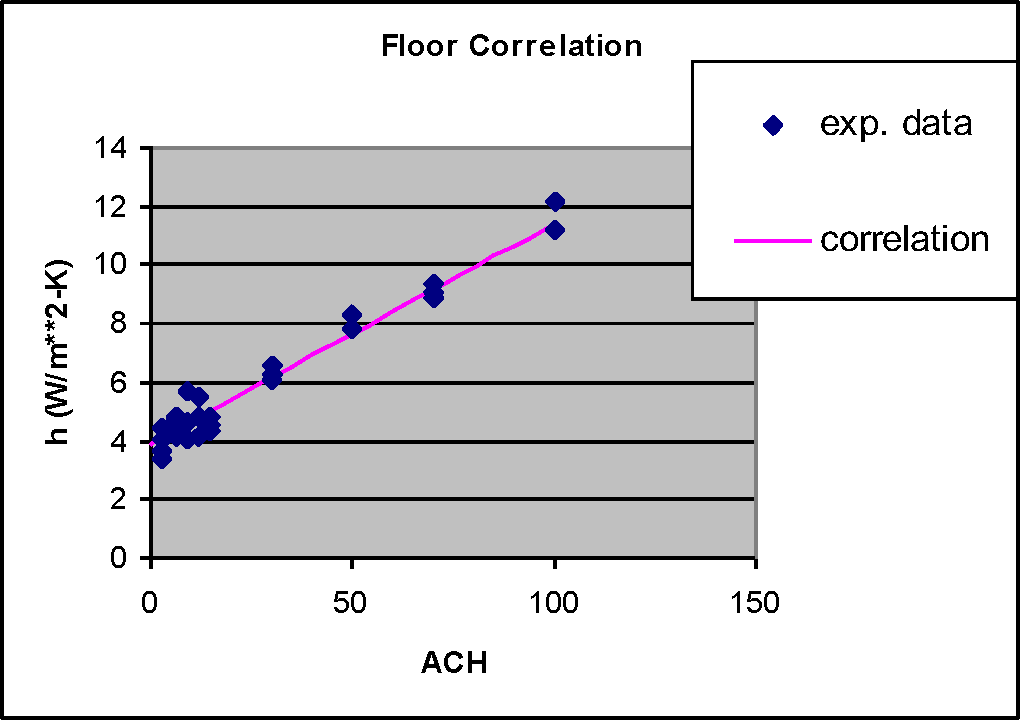
\includegraphics[width=0.9\textwidth, height=0.9\textheight, keepaspectratio=true]{media/image378.png}
\caption{Ceiling Diffuser Correlation for Floors \protect \label{fig:ceiling-diffuser-correlation-for-floors}}
\end{figure}

For ceilings:

\begin{equation}
h = 2.234 + 4.099 * AC{H^{0.503}}
\end{equation}

The correlation for ceilings is illustrated in Figure~\ref{fig:ceiling-diffuser-correlation-for-ceilings}.

\begin{figure}[hbtp] % fig 1018
\centering
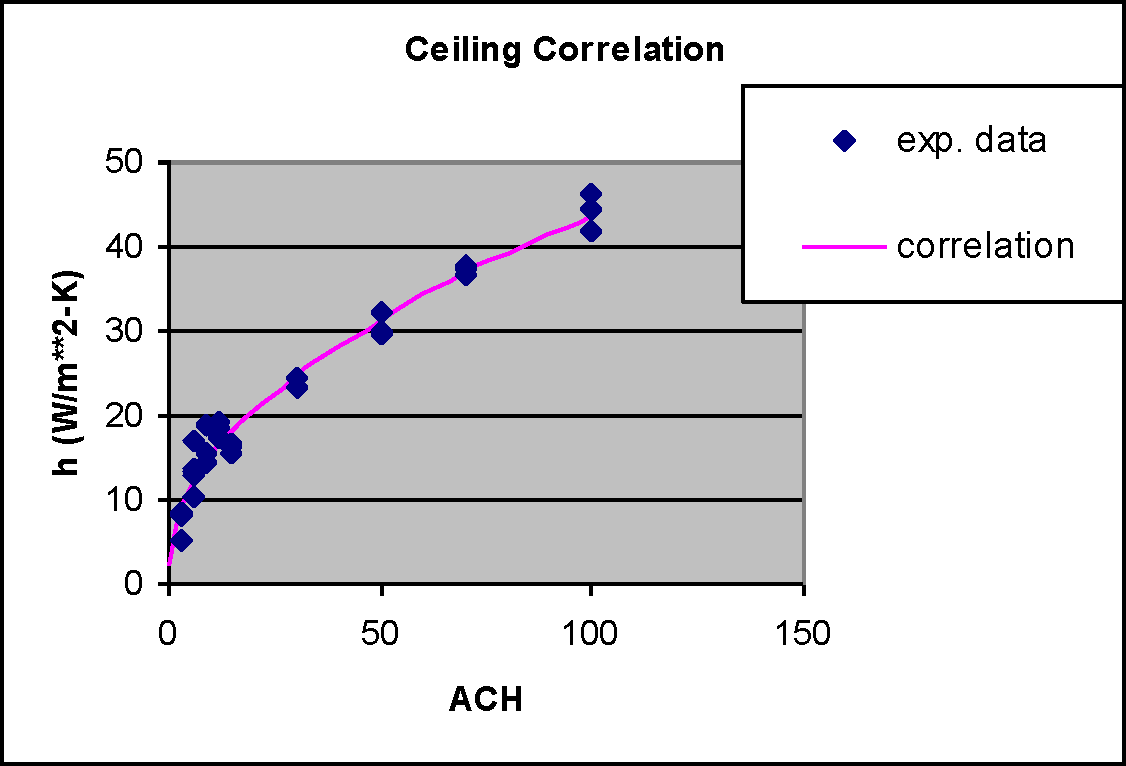
\includegraphics[width=0.9\textwidth, height=0.9\textheight, keepaspectratio=true]{media/image380.png}
\caption{Ceiling Diffuser Correlation for Ceilings \protect \label{fig:ceiling-diffuser-correlation-for-ceilings}}
\end{figure}

For Walls:

\begin{equation}
h = 1.208 + 1.012 * AC{H^{0.604}}
\end{equation}

The correlation for walls is illustrated in Figure~\ref{fig:ceiling-diffuser-correlation-for-walls}.

\begin{figure}[hbtp] % fig 1019
\centering
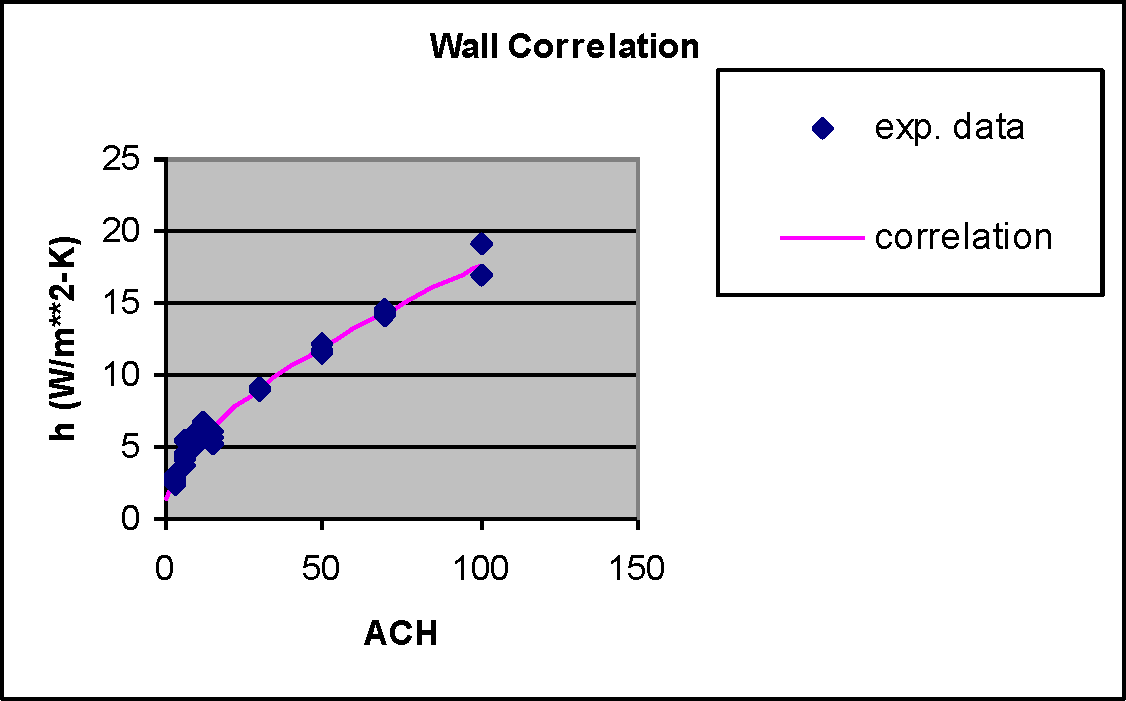
\includegraphics[width=0.9\textwidth, height=0.9\textheight, keepaspectratio=true]{media/image382.png}
\caption{Ceiling Diffuser Correlation for Walls \protect \label{fig:ceiling-diffuser-correlation-for-walls}}
\end{figure}

It should be noted that the conditions under which the correlations were developed included ACH values down to around 3.0.  So, within EnergyPlus, for ACH values of 3.0 or greater, the ceiling diffuser correlations as shown above are used.  Below ACH values of 0.5, the natural convection is determined using the TARP Algorithm (see above).  Between ACH values of 0.5 and 3.0, convection is assumed to be a mix between natural and forced convection.  Thus, between these two ACH values, EnergyPlus will use a linear interpolation between the natural convection algorithm value and the forced convection value at ACH=3.0 to avoid any discontinuities in the convection coefficient calculated and also maintain stability within the solution.

\subsubsection{Trombe Wall Algorithm}\label{trombe-wall-algorithm}

The Trombe wall algorithm is used to model convection in a ``Trombe wall zone'', i.e.~the air space between the storage wall surface and the exterior glazing.~ (See the later sections on Passive and Active Trombe Walls below for more information about Trombe walls.)~ The algorithm is identical to the convection model (based on ISO 15099) used in Window5 for convection between glazing layers in multi-pane window systems.~ The use of the algorithm for modeling an unvented Trombe wall has been validated against experimental data by Ellis (2003).

This algorithm gives the convection coefficients for air in a narrow vertical cavity that is sealed and not ventilated.~ This applies both to the air gap in between panes of a window or to the air gap between the Trombe wall glazing and the inner surface (often a selective surface).~ These convection coefficients are really the only difference between a normal zone and a Trombe zone.~ The rest of the zone heat balance is the same, e.g., transmitted solar, long-wave radiation between surfaces, etc.

For a vertical cavity, the correlation from ISO 15099 is:

\begin{equation}
\begin{array}{lcl}
    NU1 = 0.0673838 Ra^{\frac{1}{3}} & for &  5E4 < Ra < 1E6 \\
    NU1 = 0.028154 Ra^{0.4134} & for &  1E4 < Ra < 5E4 \\
    NU1 = 1 + 1.7596678E^{-10} Ra^{2.2984755} & for &  Ra \leq 1E4 \\
\end{array}
\end{equation}

\begin{equation}
{\rm{NU2}} = 0.242{\left( {{\raise0.7ex\hbox{{{\rm{Ra}}}} \!\mathord{\left/ {\vphantom {{{\rm{Ra}}} {\rm{A}}}}\right.}\!\lower0.7ex\hbox{{\rm{A}}}}} \right)^{0.272}}
\end{equation}

\begin{equation}
{\rm{NU = MAX(NU1,NU2)}}
\end{equation}

where

Nu = Nusselt number

Ra = Rayleigh number

A = aspect ratio of cavity

This is then used in EnergyPlus as follows:

Net convection coefficient from glazing to wall is:

\begin{equation}
{h_{net}} = {\rm{k}}\left( {{\raise0.7ex\hbox{{{\rm{NU}}}} \!\mathord{\left/ {\vphantom {{{\rm{NU}}} {\rm{L}}}}\right.}\!\lower0.7ex\hbox{{\rm{L}}}}} \right)
\end{equation}

where

k = conductivity of air

L = air gap thickness

Convection coefficient applied to each wall separately and actually used in the zone heat balance is:

\begin{equation}
{h_c} = 2{h_{net}}
\end{equation}

\subsubsection{ASTM C1340 Algorithm}\label{ASTM-C1340-algorithm}

The algorithm is based on ASTM C1340 Standard. This algorithm specifies to simulate heat flows in attic zone. The correlations account for the effects of surface-to-air temperature difference, heat flow direction, surface length along the heat flow direction, surface tilt angle, air speed past surface, and surface orientation. The correlations are in the form of a Nusselt number, Nu, as a function of a Rayleigh number, Ra, Grashof number, Gr, or a Reynolds number, Re. 

\begin{equation}
Nu = hL/k
\end{equation}
\begin{equation}
Ra = g \beta \rho C_p \Delta TL^3 / \nu k
\end{equation}
\begin{equation}
Gr = Ra / Pr
\end{equation}
\begin{equation}
Pr = \nu / \alpha
\end{equation}
\begin{equation}
Re = VL/ \nu
\end{equation}

\noindent 
\emph{h} = convection heat transfer coefficient \\
\emph{L} = characteristic length of surface \\
\emph{k} = thermal conductivity of air \\
\emph{g} = acceleration of gravity \\
$\beta$ = volume coefficient of expansion of air\\
$\rho$ = density of air\\
$C_p$ = specific heat of air\\
\emph{$\Delta$T} = temperature difference between surface and air\\
$\nu$ = kinematic viscosity of air\\
\emph{Pr} = Prandtl number for air\\
$\alpha$ = thermal diffusivity of air\\
\emph{V} = velocity of air stream\\

The correlations used in the model are as below. (reference: Table 1 of ASTM C1340 standard)

\begin{enumerate}
   \item Natural Convection:
   \begin{enumerate}
     \item Horizontal surface, heat flow up \\
     $Nu_n = 0.54 \: Ra^{1/4} \enspace for \enspace Ra < 8 * 10^6$ \\
     $Nu_n = 0.15 \: Ra^{1/3} \enspace for \enspace Ra > 8 * 10^6$ 
     \item Horizontal surface, heat flow down \\
     $Nu_n = 0.58 \: Ra^{0.2}$
     \item Vertical surface \\
     $Nu_n = 0.59 \: Ra^{1/4} \enspace for \enspace Ra < 1 * 10^9$ \\
     $Nu_n = 0.10 \: Ra^{1/3} \enspace for \enspace Ra > 1 * 10^9$ 
     \item Nearly horizontal surface (tilt angle less than $2^o$), heat flow down \\
     $Nu_n = 0.58 \: Ra^{0.2}$ 
     \item Tilted surfaces (greater than $2^o$ tilt), heat flow down \\
     $Nu_n = 0.56 \: (Ra \, sin (\Phi))^{1/4} \qquad  \Phi = tilt \: angle$ 
     \item Tilted surfaces, heat flow up \\
     $Nu_n = 0.56 \: (Ra \, sin (\Phi))^{1/4} \enspace for \enspace Ra/Pr < Gr_c$ \\
     $Nu_n = 0.14 \: (Ra^{1/3}- (Gr_c\,Pr)^{1/3}) \\
     \enspace + 0.56\,(Gr_c \, Pr \, sin (\Phi))^{1/4} \enspace for \enspace Ra/Pr > Gr_c$ \\
     $Gr_c = 1 * 10^6 \enspace for \enspace \Phi < 15^o $ \\
     $Gr_c = 10^{(\Phi / (1.1870\:+\:0.0870*\Phi))} \enspace for \enspace 15^o < \Phi < 75^o $ \\
     $Gr_c = 5 * 10^9 \enspace for \enspace \Phi > 75^o $
   \end{enumerate}
   \item Forced Convection: \\
   $Nu_f = 0.664 \: Pr^{1/3} \: Re^{1/2} \enspace for \enspace Re < 5 * 10^5$ \\
   $Nu_f = Pr^{1/3} \: (0.037 \: Re^{0.8} \: - 850) \enspace for \enspace Re > 5 * 10^5$
\end{enumerate}

Separate coefficients are calculated for natural and forced flow, and a mixed coefficient is calculated by taking the third root of the sum of the cubes of the two separate coefficients.

\begin{equation}
h_n = Nu_n * k / L
\end{equation}
\begin{equation}
h_f = Nu_f * k / L
\end{equation}
\begin{equation}
h_c = {(h_n^3 + h_f^3)}^{1/3}
\end{equation}

More information regarding the implemented equations in the code is provided in detail in Appendix A, section 7.7 and 7.8 of the reference: Fontanini, A. D., Aguilar, J. L. C., Mitchell, M. S., Kosny, J., Merket, N., DeGraw, J. W., and Lee, E. (2018). Predicting the performance of radiant technologies in attics: Reducing the discrepancies between attic specific and whole-building energy models. Energy and Buildings, 169, 69-83.

\subsection{Additional Heat Balance Source}\label{additional-heat-balance-source}

EnergyPlus also enables importing the pre-calculated results of other heat transfer processes to be considered in the inside heat balance calculation. An additional heat source term defined as a surface property would enable the consideration of these processes to be imported as schedules in the interior surface heat balance calculation in EnergyPlus.

The heat balance on the inside face can be written as follows:

\begin{equation}
{q''_{LWX}} + {q''_{SW}} + {q''_{LWS}} + {q''_{ki}} + {q''_{sol}} + {q''_{conv}} + {q''_{add}} = 0
\end{equation}

where:
\(q''_{add}\) = Pre-calculated results of the heat flux to the inside face from other heat transfer processes.

\subsubsection{References}\label{references-032}

Alamdari, F. and G.P. Hammond. 1983. Improved data correlations for buoyancy-driven convection in rooms.~ Building Services Engineering Research \& Technology. Vol. 4, No. 3.

ASHRAE. 1985. 1985 ASHRAE Handbook -- Fundamentals, Atlanta: American Society of Heating, Refrigerating, and Air-Conditioning Engineers, Inc.

ASHRAE. 2001. 2001 ASHRAE Handbook -- Fundamentals, Atlanta: American Society of Heating, Refrigerating, and Air-Conditioning Engineers, Inc.

ASTM International. 2015. ASTM C1340 Standard Practice for Estimation of Heat Gain or Loss Through Ceilings Under Attics Containing Radiant Barriers by Use of a Computer Program

Awbi, H.B. and A. Hatton. 1999. Natural convection from heated room surfaces. Energy and Buildings 30 (1999) 233-244.

Beausoleil-Morrison, I. 2000. The adaptive coupling of heat and air flow modeling within dynamic whole-building simulations. PhD. Thesis. University of Strathclyde, Glasgow, UK.

Ellis, Peter G. 2003. Development and Validation of the Unvented Trombe Wall Model in EnergyPlus. Master's Thesis, University of Illinois at Urbana-Champaign.

Fisher, D.E. and C.O. Pedersen. 1997. ``Convective Heat Transfer in Building Energy and Thermal Load Calculations'', ASHRAE Transactions, Vol. 103, Pt. 2.

Fohanno, S., and G. Polidori. 2006. Modelling of natural convective heat transfer at an internal surface. Energy and Buildings 38 (2006) 548 - 553

Fontanini, A. D., Aguilar, J. L. C., Mitchell, M. S., Kosny, J., Merket, N., DeGraw, J. W., and Lee, E. (2018). Predicting the performance of radiant technologies in attics: Reducing the discrepancies between attic specific and whole-building energy models. Energy and Buildings, 169, 69-83.

Goldstein, K. and A. Novoselac. 2010. Convective Heat Transfer in Rooms With Ceiling Slot Diffusers (RP-1416). \emph{HVAC\&R Research Journal} TBD

Karadag, R. 2009. New approach relevant to total heat transfer coefficient including the effect of radiation and convection at the ceiling in a cooled ceiling room. Applied Thermal Engineering 29 (2009) 1561-1565

Khalifa AJN. 1989. Heat transfer processes in buildings. Ph.D.~Thesis, University of Wales College of Cardiff, Cardiff, UK.

ISO. 2003. ISO 15099:2003. Thermal performance of windows, doors, and shading devices -- Detailed calculations. International Organization for Standardization.

Walton, G. N. 1983. Thermal Analysis Research Program Reference Manual. NBSSIR 83-2655. National Bureau of Standards (now NIST). This is documentation for ``TARP.''
